\documentclass{beamer}
\usepackage{graphicx}
\usepackage{listings}

\title{Template Metaprogramming}
\subtitle{Or: How I Learned to Stop Worrying and Love the Angle Brackets}
\author{Murray Colpman}

\AtBeginSection[]
{
  \begin{frame}
    \frametitle{Table of Contents}
    \tableofcontents[currentsection]
  \end{frame}
}

\begin{document}
\lstset{language=C++,
                basicstyle=\ttfamily,
                keywordstyle=\color{blue}\ttfamily,
                stringstyle=\color{red}\ttfamily,
                commentstyle=\color{green}\ttfamily,
                morecomment=[l][\color{magenta}]{\#}
}

  \frame{\titlepage}
  \section{Intro}
  \begin{frame}
    \frametitle{WHY?!}
    \begin{itemize}
      \pause
      \item Adds a lot more power to generic programming
        \pause
        \begin{itemize}
          \item Useful for writing libraries, generally used over Java's
            dynamic polymorphism pattern where convenient
          \pause
          \item Implement static polymorphism (Curiously Recurring Template
            Pattern)
        \end{itemize}
      \pause
      \item Run code evaluable at compile time at compile time.
      \pause
      \item Harness the true power of the type checker
      \pause
      \item Terrify and impress people
    \end{itemize}
  \end{frame}
  \begin{frame}
    \frametitle{WHY?! (cont'd)}
    Templates are free at runtime in terms of time complexity, but do add to
    binary size.
    
    \pause

    They might also add to compile time, but is that really a bad thing?

    \pause

    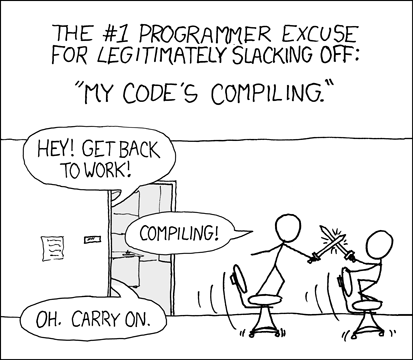
\includegraphics[height=0.5\textheight]{compiling} % magic
  \end{frame}
  \begin{frame}
    \frametitle{Some notes}
    \begin{itemize}
      \pause
      \item Mostly covering C++03
      \pause
      \item Assumes you remember our template lecture
      \pause
      \item I'm not an expert
    \end{itemize}
  \end{frame}
  \section{Template Metaprogramming Theory}
  \begin{frame}[fragile]
    \frametitle{What is TMP?}
    \pause
    It was recognised that people needed to commit atrocities using macros in
    order to get sensible generic programming in the earliest versions of C++.
    \pause

    \begin{lstlisting}
#define TYPE int
#include <insanity.h>
#undef TYPE

#define TYPE double
#include <insanity.h>
#undef TYPE
    \end{lstlisting}

    \begin{itemize}
      \pause
      \item Templates were introduced to make the world a less horrible place.
      \pause
      \item Templates are flexible and Turing-complete.
      \pause
      \item Template metaprogramming is the use of these more advanced features
        of templates to produce code at compile-time.
      \pause
      \item Template metaprogramming is a functional language(!)
    \end{itemize}
\end{frame}
  \begin{frame}
    \frametitle{Mappings to functional languages}
    \begin{itemize}
        \pause
        \item Variables represented by static const or enum values
        \pause
        \item References represented by typedefs
        \pause
        \item Branching uses template specialisation as pattern matching
        \pause
        \item Iteration works like recursion
    \end{itemize}
  \end{frame}
  \section{Examples}
  \section{SFINAE}
  \section{C++11 Improvements}
\end{document}
